\section{Design and Reconstruction of the CMS HGCAL}
\label{sec:hgcal:design}


\begin{figure}[ht]
    \centering
    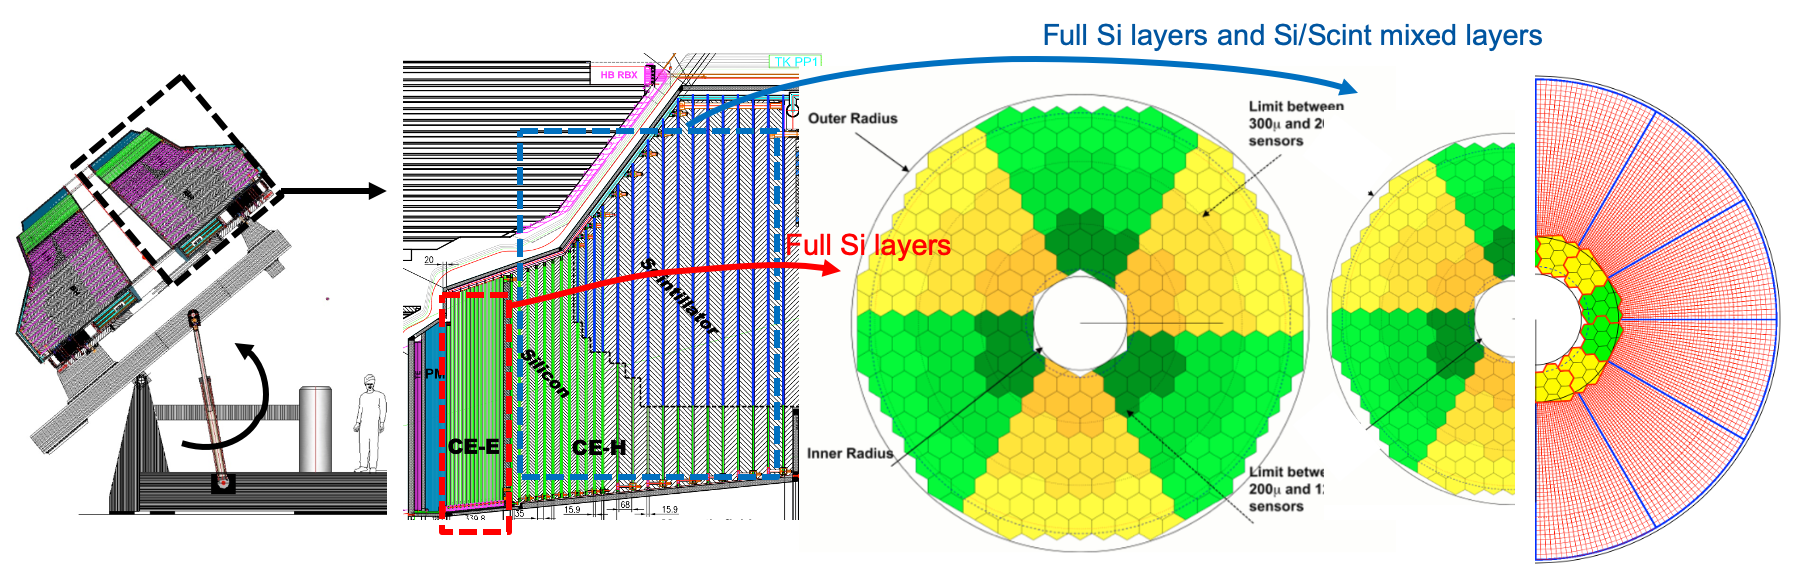
\includegraphics[trim=0cm 0cm 0cm 0cm, clip,width=0.99\textwidth]{chapters/HGCal/figures/chep/hgcal2.png} 
    \caption{ The design of HGCAL \cite{Collaboration:2293646}. (\emph{left}) Sketch of HGCAL endcap. (\emph{mid-left}) The internal structure on the longitudinal-radial (z-r) plane. Red and blue rectangles indicate regions of CE-E (for calorimeter endcap electromagnetic) and CE-H (for calorimeter endcap hadronic), respectively, where CE-E has 28 full Si layers and CE-H has 8 full Si layers plus 14 Si-scintillators hybrid layers. (\emph{mid-right, right}) Layouts of CE-E and CE-H layer. Silicon wafers are shown as yellow and green hexagons and scintillators are shown as red mesh. Darker, medium and lighter shades of hexagons represent silicon wafers with thickness of 120, 200 and 300 $\mu$m, respectively.
    }
    \label{fig:hgcal}
\end{figure}

% HGCAL design
The design of HGCAL \cite{Collaboration:2293646} is shown in Figure~\ref{fig:hgcal}. Two HGCAL endcaps will be mounted on both sides of the CMS detector. Each endcap weighs about 215 tons and measures about 2 m in longitudinal direction and 2.3 m in radial direction, covering $1.5<|\eta|<3.0$. The full system operates at a temperature of $-35^\circ$C maintained by a CO$_2$ cooling system. Each endcap consists of 50 layers, each of which combines passive absorber material and active sensor material. The front 28 layers are the electromagnetic part (CE-E), which uses Cu, CuW and Pb as absorber and Si wafers with 120, 200, 300 $\mu$m thickness as sensors. The back 22 layers are the hadronic part (CE-H), which uses stainless steel and Cu as absorber and includes 8 full Silicon layers plus 14 hybrid layers of Si sensors and plastic scintillators with SiPM readout. The electromagnetic radiation thickness and hadronic interaction thickness of CE-E are $25 X_0$ and $1.3 \lambda$ respectively, while the hadronic interaction thickness of CE-H is $8.2 \lambda$. In total, The full HGCAL system has 620 m$^2$ of Silicon and about 400 m$^2$ of plastic scintillators. The size of each Si sensor is 0.5-1.0 cm$^2$ and the number of Si channels is about 6 million. The size of the scintillators is 4-30 cm$^2$ and the number of scintillator channels is about 240 thousand.


% HGCAL reconstruction
As a consequence of both high pile-up in the HL-LHC and enormous number of channels in the HGCAL, the number of input hits to HGCAL clustering algorithm is huge, usually in the order of $n\sim O(10^5)$ in PU200 events, where $n$ denotes the number of hits. The clustering algorithm aggregates hits in 2D clusters layer by layer, producing about $k \sim O(10^4)$ clusters, where $k$ denotes number of clusters. The average number of hits in a cluster is about $m=n/k \sim 10$; therefore HGCAL clustering task is characterized by $n> k \gg m$. Since cells are small compared to shower lateral size, an "energy density" is defined to better hint regional energy blobs in the HGCAL clustering. After 2D clustering algorithm, 3D showers in HGCAL are reconstructed by collecting and associating 2D clusters on different layers using TICL algorithms \cite{ticlwebsite}. 

% time budget
The current trigger system in CMS consists of two levels: Level 1 Trigger (L1T) and High Level Trigger (HLT). L1T utilizes customized ASICs and FPGAs to reduce the event rate from 40 MHz LHC collision frequency to 100 kHz within a 4 $\mu$s time budget for decision; HLT is fully based on C++ software running on CPUs and further reduces event rate from 100 kHz to 1 kHz with a 300 ms time budget for decision. However, in the era of HL-LHC, CMS HLT expects 30 times more computing load: 1.3x from upgraded detectors with more channels; 3x from increased number of pile-up interactions; 7.5x from improved L1T output rate. Among this 30x surge of the computing demand, improvement in the CPU performance by 2026 is expected to account for only 4x. Therefore, there will be a considerable deficit of computing power if the HLT architecture remains unchanged in 2026. In the HL-LHC era, the HLT time budget for CMS HGCAL clustering is roughly estimated to be less than a few tens of milliseconds. It is particularly a huge challenge of computing for the HGCAL clustering algorithm to process $n\sim5\times10^5$ hits within such a limited time budget. To cope with this computing challenge, CMS is studying the feasibility of heterogeneous computing in HLT and offline reconstruction. With the support of CUDA \cite{nvidia2011nvidia} in the CMS software framework (CMSSW), it is possible to accelerate the HGCAL reconstruction with GPUs. 